The client side is implemented as an Android application, \textit{DMDataGenerator}, that gathers location data for its users, interracts with the server and, if needed, it communicates a possible \textit{safe location} to the user.Taking into consideration the fact that we have developed this client application as an easy way of testing the underlying management algorithm, there are multiple ways of using it, as a user but also as a developer:
\begin{itemize}
\item Generate data samples
\item Combine data samples into custom new ones
\item Replay samples
\item Choose preferences in terms of what means a \textit{safe location}
\item Choose friends
\end{itemize}

In the next paragraphs we will briefly describe each one of these....

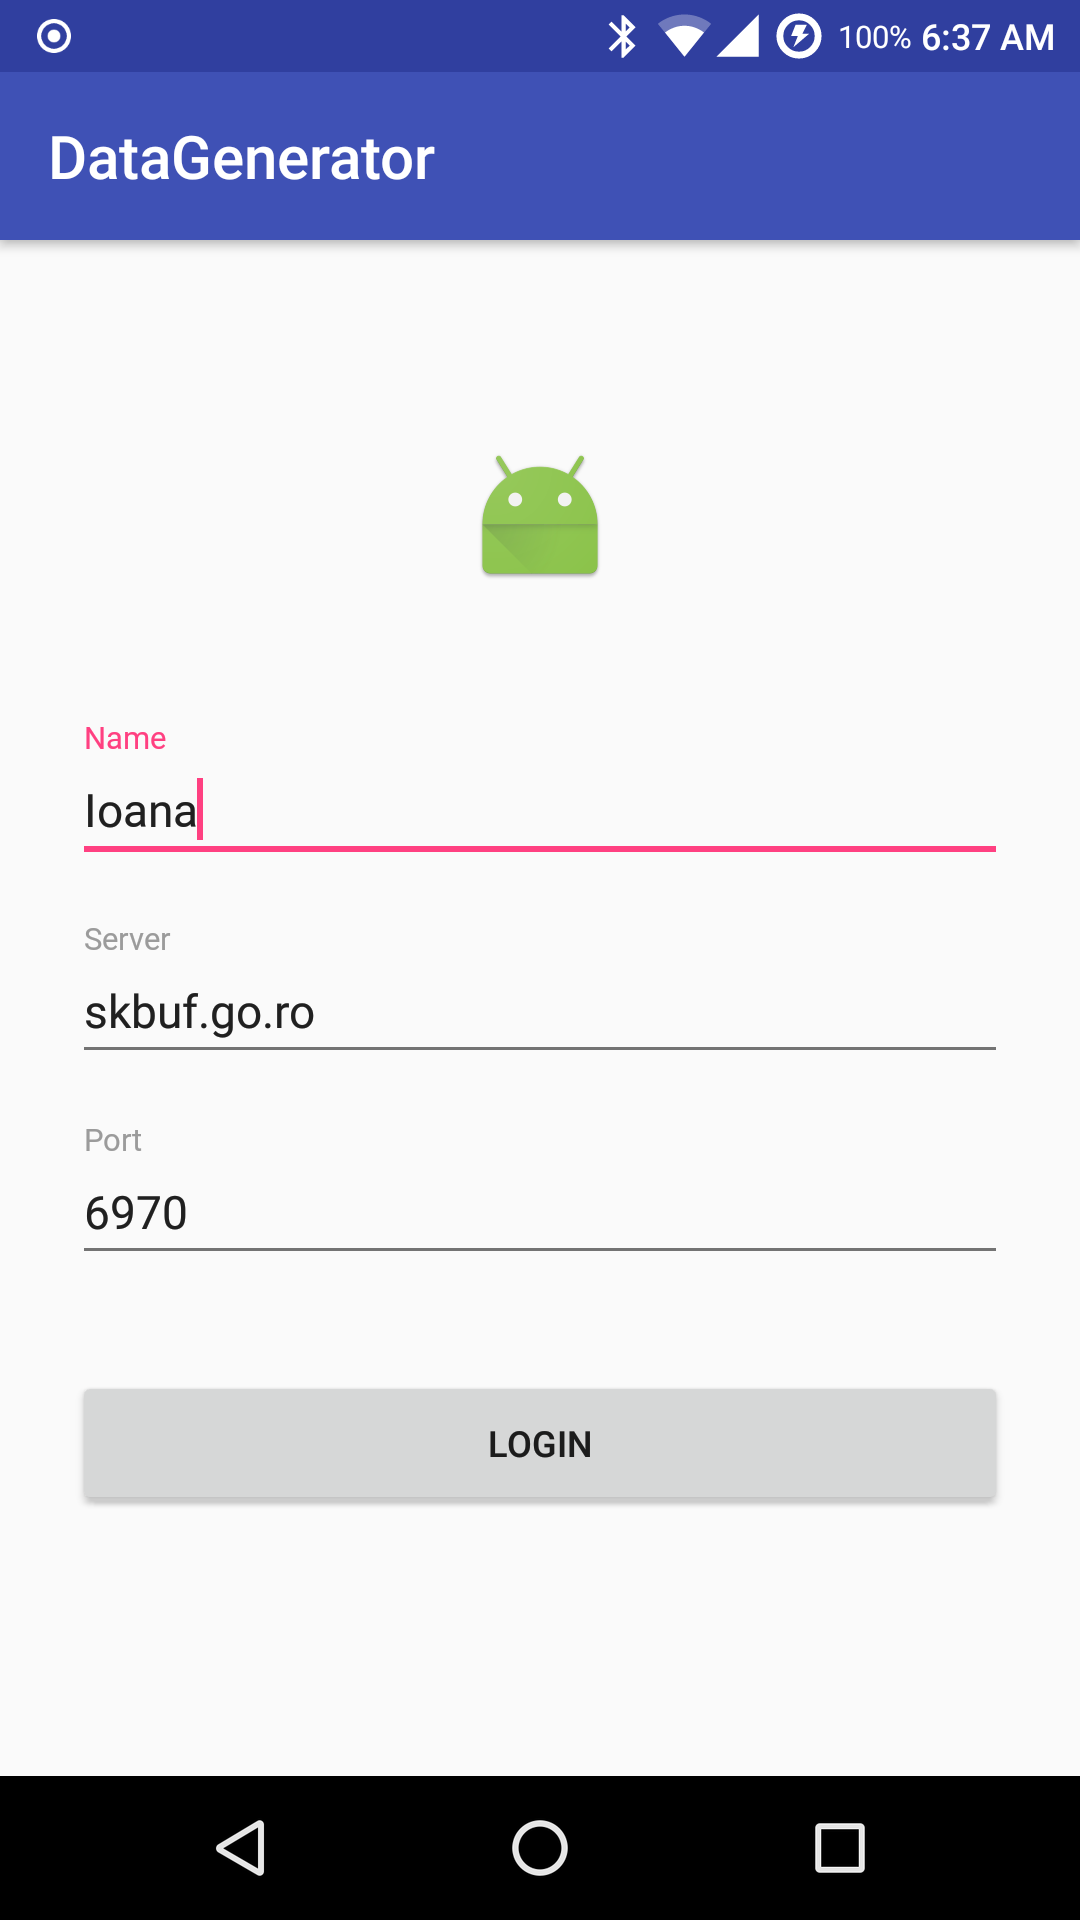
\includegraphics[scale=0.09]{login}
